\documentclass[10pt]{exam}
\usepackage[pdftex]{graphicx, color}

\usepackage{amsmath}
\usepackage{minted}


\usepackage{tikz}
\usetikzlibrary{automata,positioning}
\tikzset{
    state/.style={
           rectangle,
           rounded corners,
           draw=black, very thick,
           minimum height=2em,
           inner sep=2pt,
           text centered,
           },
}
\headheight 8pt \headsep 20pt \footskip 30pt
\textheight 9in \textwidth 6.5in
\oddsidemargin 0in \evensidemargin 0in
\topmargin -.35in

\newcommand {\pts}[1]{({\bf #1 pts})}

\begin{document}
\begin{center}
  \Large CS131 Compilers: Writing Assignment 2\\Due Sunday, April 3, 2021 at 23:59pm
\end{center}

\begin{center}
  %% Change this:
  \LARGE Tian Haoyuan - 2020533013
\end{center}

This assignment asks you to prepare written answers to questions on
context-free grammars and parsing. Each of the questions has a short answer. You
may discuss this assignment with other students and work on the problems
together. However, your write-up should be your own individual work.
and you should indicate in your submission who you worked with, if applicable.
Written assignments are turned in at the start of lecture.
You should use the Latex template provided at the course web site to write your solution.
\\
Sample for \texttt{tikz} DFA:

\begin{center}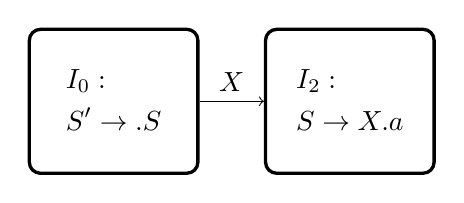
\begin{tikzpicture}
    \node[state] (I0) {
      \parbox{2cm}{\begin{equation*}\begin{aligned}
             & I_0:              \\
             & S' \rightarrow .S \\
          \end{aligned}\end{equation*}}
    };

    \node[state, right of=I0, node distance=3cm] (I1){
      \parbox{2cm}{\begin{equation*}\begin{aligned}
             & I_2:             \\
             & S\rightarrow X.a \\
          \end{aligned}\end{equation*}}
    };

    \path[->]
    (I0) 	edge 					node[above]{$X$} (I1);

  \end{tikzpicture}\end{center}
Sample for \texttt{tikz} Tree:
\begin{center}\begin{tikzpicture}    [
      level distance = 4em,
      level 1/.style={sibling distance=3cm},
      level 2/.style={sibling distance=2cm},
      level 3/.style={sibling distance=1.5cm}
    ]
    \node(root){expr}
    child{node{\textbf{while}}}
    child{node{expr}
        child{node{\textbf{not}}}
      }
    child{node{\textbf{loop}}}
    child{node{expr}
        child{node{\textbf{ID}}}
        child{node{$\leftarrow$}}
        child{node{expr}}
      };

  \end{tikzpicture}\end{center}
\begin{center}
  %% Change this:
  I worked with: nobody
\end{center}

\begin{enumerate}
  \item  \pts{$2*3+4 = 10$} Give context-free grammar (CFG) for each of the following languages, for the last
        part, you don't need to draw the tree but the semantic alongside with the production rule:
        \begin{enumerate}
          \item The alphabet is $\{1,2,-, *\}$, all strings of the valid products of integers that is smaller
                than 0.
                \textcolor{blue}{
                  \[\begin{array}{cll}
                      %% Your answer here
                      E & \rightarrow & N*P|P*N      \\
                      N & \rightarrow & E|-P         \\
                      P & \rightarrow & N*N|P*P|D    \\
                      D & \rightarrow & (1|2)D|(1|2)
                    \end{array}\]}
          \item The alphabet is \texttt{\{[,],\{,\},} \textbf{,} \texttt{\}}, all strings of the valid comma
                separated sets and list. There must exist one element in set or list.
                \textcolor{blue}{\[
                    %% Your answer here
                    \begin{array}{cll}
                      S & \rightarrow & \{T\}|[T]      \\
                      T & \rightarrow & T,T|S|\epsilon
                    \end{array}
                  \]}

          \item The alphabet is $\{0,1\}$, all strings of the number of 1 's is at most two more than the
                number of 0 's.
                \textcolor{blue}{\[
                    %% Your answer here
                    \begin{array}{cll}
                      E & \rightarrow & ZSZ1ZSZ1ZSZ|ZSZ1ZSZ|ZSZ \\
                      S & \rightarrow & 0S1S|1S0S|\epsilon      \\
                      Z & \rightarrow & 0Z|\epsilon
                    \end{array}
                  \]}
          \item All regular languages can be described by a context free grammar, but the converse is not true.
                Can we write a CFG that translate all five core regular expressions(epsilon, character concatenation, union,
                Kleene star)?

                For any regular expression $R$, your translation should construct a CFG $G$ such that the languages of
                $R$ and $G$ are equal. Fill in the right-hand sides of the productions below.

                \textcolor{blue}{\[
                    %% Your answer here
                    \begin{array}{cll}
                      S_{\epsilon}     & \rightarrow & \epsilon                  \\
                      S_{c \in \Sigma} & \rightarrow & c                         \\
                      S_{A B}          & \rightarrow & A\ B                      \\
                      S_{A+B}          & \rightarrow & A\ |\ B                   \\
                      S_{A^{*}}        & \rightarrow & A\ S_{A^{*}}\ |\ \epsilon
                    \end{array}
                  \]}

        \end{enumerate}



  \item \pts{$3\times 3= 9$} Consider the following CFG.
        \[\begin{array}{cll}
            S & \rightarrow & S a S \mid U     \\
            U & \rightarrow & U u U \mid T     \\
            T & \rightarrow & t|f| T n \mid(S) \\
          \end{array}\]

        \begin{enumerate}
          \item Is the grammar as given ambiguous? If yes, give an example of an expression
                with two parse trees under this grammar. If not, explain why that is the case.\\
                \textcolor{blue}{
                  It is ambiguous.\\
                  Example: tatat\\
                  \begin{tikzpicture}    [
                      level distance = 2.5em,
                      level 1/.style={sibling distance=2cm},
                      level 2/.style={sibling distance=2cm},
                      level 3/.style={sibling distance=1.5cm}
                    ]
                    \node(root){S}
                    child{node{S}
                        child{node{S}
                            child{node{U}
                                child{node{T}
                                    child{node{\textbf{t}}}
                                  }
                              }
                          }
                        child{node{\textbf{a}}}
                        child{node{S}
                            child{node{U}
                                child{node{T}
                                    child{node{\textbf{t}}}
                                  }
                              }
                          }
                      }
                    child{node{\textbf{a}}
                      }
                    child{node{S}
                        child{node{U}
                            child{node{T}
                                child{node{\textbf{t}}}
                              }
                          }
                      };
                  \end{tikzpicture}
                  \begin{tikzpicture}    [
                      level distance = 2.5em,
                      level 1/.style={sibling distance=2cm},
                      level 2/.style={sibling distance=2cm},
                      level 3/.style={sibling distance=1.5cm}
                    ]
                    \node(root){S}
                    child{node{S}
                        child{node{U}
                            child{node{T}
                                child{node{\textbf{t}}}
                              }
                          }
                      }
                    child{node{\textbf{a}}
                      }
                    child{node{S}
                        child{node{S}
                            child{node{U}
                                child{node{T}
                                    child{node{\textbf{t}}}
                                  }
                              }
                          }
                        child{node{\textbf{a}}}
                        child{node{S}
                            child{node{U}
                                child{node{T}
                                    child{node{\textbf{t}}}
                                  }
                              }
                          }
                      };
                  \end{tikzpicture}
                }
          \item Transform the CFG given above by eliminating ambiguity and
                left recursion, if needed.
                \textcolor{blue}{\[\begin{array}{cll}
                      S  & \rightarrow & U\ S'                           \\
                      S' & \rightarrow & a\ U\ S'\ |\ \epsilon           \\
                      U  & \rightarrow & T\ U'                           \\
                      U' & \rightarrow & u\ T\ U'\ |\ \epsilon           \\
                      T  & \rightarrow & t\ T'\ |\ f\ T'\ |\ (\ S\ )\ T' \\
                      T' & \rightarrow & n\ T'\ |\ \epsilon
                    \end{array}\]}
          \item What advantage does left recursion have over right recursion in shift-reduce parsing?\\
                \textcolor{blue}{
                  In shift-reduce parsing, right recursion requires immediate decision on whether to shift or to reduce when it encounters a specific nonterminal,
                  while left recursion only have one option. \\
                  For example, consider left recursion $A\rightarrow Aa|a$ and right recursion $A\rightarrow aA|a$,
                  which are obviously equivalent. With left recursion $A\rightarrow Aa|a$, the parser would only have one option when the top of the stack (or the immediate input token) is either A or a, while with right recursion $A\rightarrow aA|a$,
                  the parser (LR(0)) would have a shift-shift conflict with input a, and it may need SLR or LR.
                }
        \end{enumerate}

  \item \pts{$3\times 3= 9$} Consider the following CFG.
        \[\begin{array}{cll}
            E & \rightarrow & ( \ T     \\
            T & \rightarrow & Q \ )     \\
            Q & \rightarrow & q \ A \ q \\
            A & \rightarrow & a \ A     \\
            A & \rightarrow & \epsilon
          \end{array}\]

        \begin{enumerate}
          \item Compute the Nullable, First and Follow sets for the grammar.\\
                \textcolor{blue}{
                  $Nullable(E)=false,Nullable(T)=false,Nullable(Q)=false,Nullable(A)=true,$\\
                  $First(E)=\{(\},First(T)=\{q\},First(Q)=\{q\},First(A)=\{a,\epsilon\},$\\
                  $Follow(E)=\{\$\},Follow(T)=\{\$\},Follow(Q)=\{)\},Follow(A)=\{q\}.$
                }
          \item Give the LL(1) parsing table for the grammar.\\
                \textcolor{blue}{
                  \begin{tabular}{|c|c|c|c|c|c|}
                    \hline
                      & (                & ) & q                  & a                 & \$ \\
                    \hline
                    E & $E\rightarrow(T$ &   &                    &                   &    \\
                      \hline
                    T &                  &   & $T\rightarrow Q)$  &                   &    \\
                    \hline
                    Q &                  &   & $Q\rightarrow qAq$ &                   &    \\
                    \hline
                    A &                  &   & $A\rightarrow q$   & $A\rightarrow aA$ &    \\
                    \hline
                  \end{tabular}
                }
          \item Is this grammar LALR(1)? Give your reason if it is not LALR(1), otherwise give the LALR(1) parsing table
                for the grammar.\\
                \textcolor{blue}{
                  \[\begin{array}{cll}
                      1. \ E & \rightarrow & ( \ T     \\
                      2. \ T & \rightarrow & Q \ )     \\
                      3. \ Q & \rightarrow & q \ A \ q \\
                      4. \ A & \rightarrow & a \ A     \\
                      5. \ A & \rightarrow & \epsilon
                    \end{array}\]
                  \begin{tabular}{|c|c|c|c|c|c|||c|c|c|c|}
                    \hline
                       & (  & )  & q  & a  & \$  & E & T & Q & A  \\
                    \hline
                    0  & s2 &    &    &    &     & 1 &   &   &    \\
                    \hline
                    1  &    &    &    &    & acc &   &   &   &    \\
                    \hline
                    2  &    &    & s5 &    &     &   & 3 & 4 &    \\
                    \hline
                    3  &    &    &    &    & r1  &   &   &   &    \\
                    \hline
                    4  &    & s7 &    &    &     &   &   &   &    \\
                    \hline
                    5  &    &    &    & s8 &     &   &   &   & 7  \\
                    \hline
                    6  &    &    &    &    & r2  &   &   &   &    \\
                    \hline
                    7  &    &    & s9 &    &     &   &   &   &    \\
                    \hline
                    8  &    &    & r5 & s8 &     &   &   &   & 10 \\
                    \hline
                    9  &    & r3 &    &    &     &   &   &   &    \\
                    \hline
                    10 &    &    & r4 &    &     &   &   &   &    \\
                    \hline
                  \end{tabular}\\
                  It is LALR(1).
                }
        \end{enumerate}

  \item \pts{$8$}  Using the context-free grammar for ChocoPy given in the ChocoPy
        manual, draw a parse tree for the following expression.

        \begin{minted}[mathescape, linenos]{python}
while (x == 1 < 2):
    y = z + 2 * x + 1
\end{minted}
        Note that the context-free grammar by itself is ambiguous, so you will
        need to use the precedence and associativity rules.
        \textcolor{blue}{
          %% Your answer here
          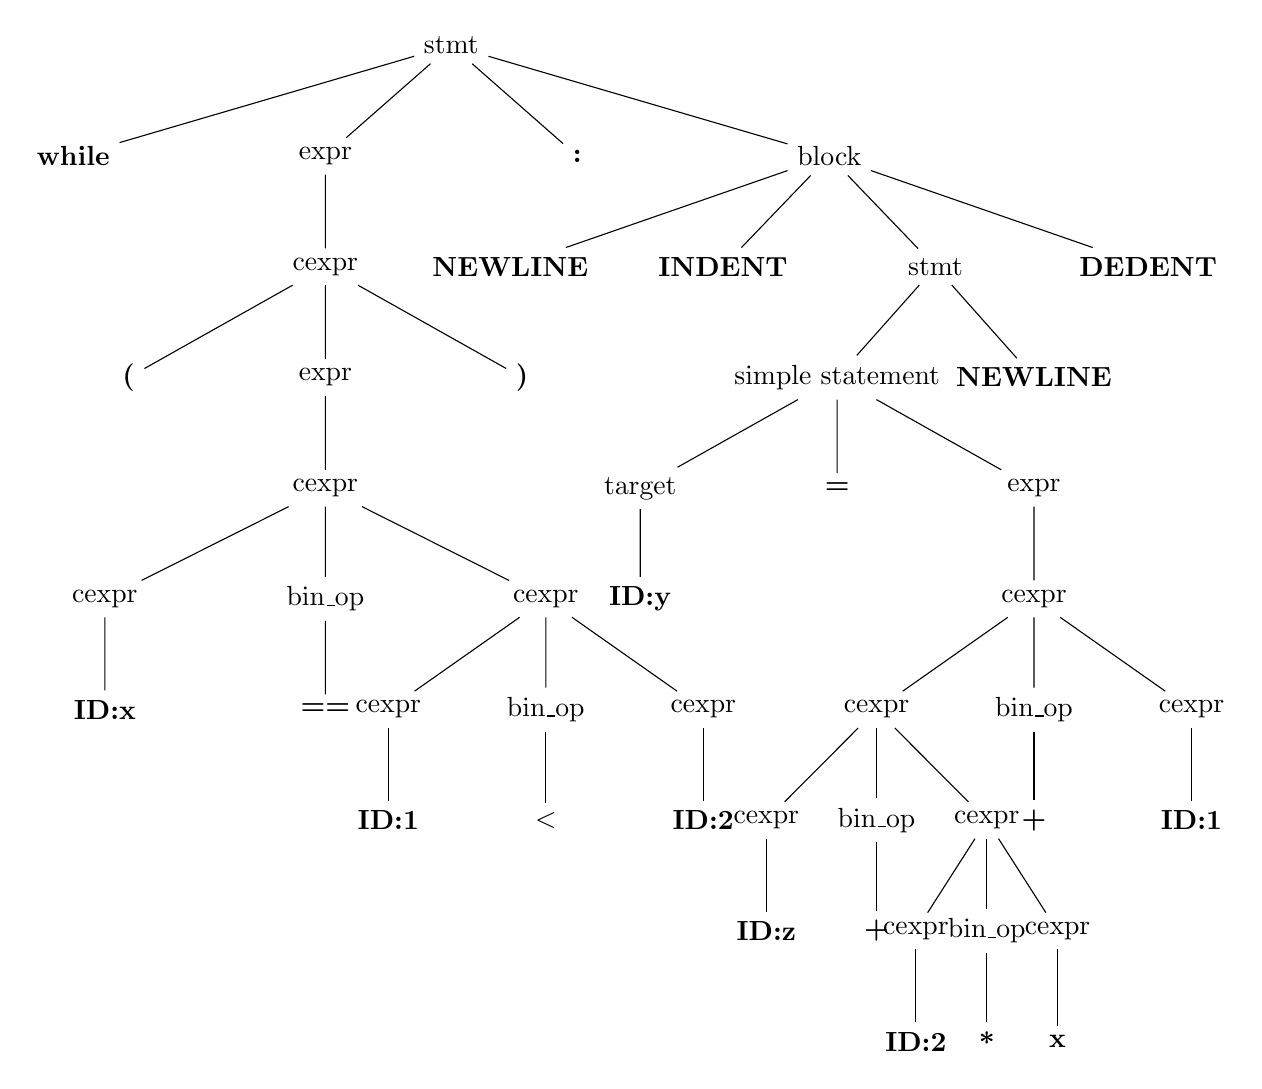
\begin{tikzpicture}[
              level distance = 4em,
              level 1/.style={sibling distance=3.2cm},
              level 2/.style={sibling distance=2.7cm},
              level 3/.style={sibling distance=2.5cm},
              level 4/.style={sibling distance=2.5cm},
              level 5/.style={sibling distance=2.8cm},
              level 6/.style={sibling distance=2.0cm},
              level 7/.style={sibling distance=1.4cm},
              level 8/.style={sibling distance=0.9cm}
            ]
            \node(root){stmt}
            child{node{\textbf{while}}}
            child{node{expr}
                child{node{cexpr}
                    child{node{\textbf{(}}}
                    child{node{expr}
                        child{node{cexpr}
                            child{node{cexpr}
                                child{node{\textbf{ID:x}}}}
                            child{node{bin\_op}
                                child{node{\textbf{==}}}}
                            child{node{cexpr}
                                child{node{cexpr}
                                    child{node{\textbf{ID:1}}}}
                                child{node{bin\_op}
                                    child{node{\textbf{$<$}}}}
                                child{node{cexpr}
                                    child{node{\textbf{ID:2}}}}
                              }
                          }
                      }
                    child{node{\textbf{)}}}
                  }
              }
            child{node{\textbf{:}}}
            child{node{block}
                child{node{\textbf{NEWLINE}}}
                child{node{\textbf{INDENT}}}
                child{node{stmt}
                    child {node{simple statement}
                        child{node{target}
                            child{node{\textbf{ID:y}}}
                          }
                        child{node{\textbf{=}}}
                        child{node{expr}
                            child{node{cexpr}
                                child{node{cexpr}
                                    child{node{cexpr}
                                        child{node{\textbf{ID:z}}}
                                      }
                                    child{node{bin\_op}
                                        child{node{\textbf{+}}}}
                                    child{node{cexpr}
                                        child{node{cexpr}
                                            child{node{\textbf{ID:2}}}}
                                        child{node{bin\_op}
                                            child{node{\textbf{*}}}}
                                        child{node{cexpr}
                                            child{node{\textbf{x}}}}
                                      }
                                  }
                                child{node{bin\_op}
                                    child{node{\textbf{+}}}}
                                child{node{cexpr}
                                    child{node{\textbf{ID:1}}}}
                              }
                          }
                      }
                    child {node{\textbf{NEWLINE}}}
                  }
                child{node{\textbf{DEDENT}}}
              };
          \end{tikzpicture}
        }

  \item \pts{$4\times 4 =16$} Consider the following grammar describing a simplified programming language:
        \[\begin{array}{cll}
            P & \rightarrow & \epsilon          \\
            P & \rightarrow & E \ ;             \\
            E & \rightarrow & 1                 \\
            E & \rightarrow & E \ + \ E         \\
            E & \rightarrow & E \ \times \ E    \\
            E & \rightarrow & E \ ? \ E \ : \ E \\
            E & \rightarrow & ( \ E \ )
          \end{array}\]

        $P$ and $E$ are nonterminals, while others are terminals.
        \begin{enumerate}
          \item Give the First and Follow sets for each nonterminal in the grammar.\\
                \textcolor{blue}{
                  $First(E)=\{1,(\},First(P)=\{\epsilon,1,(\}$\\
                  $Follow(E)=\{;,+,\times,?,:,)\},Follow(P)=\{\$\}$
                }
          \item Using this information, produce an (improper) LL(1) parsing table for this grammar. It’s improper because
                some slots will have more than one production.\\
                \textcolor{blue}{\[\begin{array}{cll}
                      1.\  P & \rightarrow & \epsilon          \\
                      2.\  P & \rightarrow & E \ ;             \\
                      3.\  E & \rightarrow & 1                 \\
                      4.\  E & \rightarrow & E \ + \ E         \\
                      5.\  E & \rightarrow & E \ \times \ E    \\
                      6.\  E & \rightarrow & E \ ? \ E \ : \ E \\
                      7.\  E & \rightarrow & ( \ E \ )
                    \end{array}\]
                  \begin{tabular}{|c|c|c|c|c|c|c|c|c|c|}
                    \hline
                      & 1       & (       & ) & ; & + & $\times$ & ? & : & \$ \\
                    \hline
                    E & 3,4,5,6 & 4,5,6,7 &   &   &   &          &   &   &    \\
                    \hline
                    P & 2       & 2       &   &   &   &          &   &   & 1  \\
                    \hline
                  \end{tabular}
                }
          \item Modify the grammar to be LL(1) (unambiguous and with at most one production per
                table entry).\\
                \textcolor{blue}{
                  \[\begin{array}{cll}
                      P  & \rightarrow & \epsilon                   \\
                      P  & \rightarrow & E \ ;                      \\
                      E  & \rightarrow & B \ ? \ E \ : \ E\ |\ B    \\
                      B  & \rightarrow & T\ B'                      \\
                      B' & \rightarrow & +\ T\ B'\ |\ \epsilon      \\
                      T  & \rightarrow & F\ T'                      \\
                      T' & \rightarrow & \times\ F\ T'\ |\ \epsilon \\
                      F  & \rightarrow & (\ E\ )\ |\ 1
                    \end{array}\]
                }
          \item repeat part (a),(b) with your result of part (c).\\
                \textcolor{blue}{
                  $First(E)=First(T)=First(F)=First(B)=\{1,(\},First(T')=\{\times, \epsilon\},\\First(B')=\{+,\epsilon\},First(P)=\{\epsilon,1,(\},$\\
                  $Follow(P)=\{\$\},Follow(E)=\{;,),:\},\\Follow(B)=Follow(B')=\{;,),:,?\},\\Follow(T)=Follow(T')=\{+,;,),:,?\},Follow(F)=\{\times,+,;,),:,?\}.$\\
                  \[\begin{array}{cll}
                      \ 1.\ P  & \rightarrow & \epsilon          \\
                      \ 2.\ P  & \rightarrow & E \ ;             \\
                      \ 3.\ E  & \rightarrow & B \ ? \ E \ : \ E \\
                      \ 4.\ E  & \rightarrow & B                 \\
                      \ 5.\ B  & \rightarrow & T\ B'             \\
                      \ 6.\ B' & \rightarrow & +\ T\ B'\         \\
                      \ 7.\ B' & \rightarrow & \epsilon          \\
                      \ 8.\ T  & \rightarrow & F\ T'             \\
                      \ 9.\ T' & \rightarrow & \times\ F\ T'     \\
                      10.\ T'  & \rightarrow & \epsilon          \\
                      11.\ F   & \rightarrow & (\ E\ )           \\
                      12.\ F   & \rightarrow & 1
                    \end{array}\]
                  \begin{tabular}{|c|c|c|c|c|c|c|c|c|c|}
                    \hline
                       & 1  & (  & )  & ;  & +  & $\times$ & ?  & :  & \$ \\
                    \hline
                    P  & 2  & 2  &    &    &    &          &    &    & 1  \\
                    \hline
                    E  & 3  & 3  &    &    &    &          &    &    &    \\
                    \hline
                    B  & 5  & 5  &    &    &    &          &    &    &    \\
                    \hline
                    B' &    &    & 7  & 7  & 6  &          & 7  & 7  &    \\
                    \hline
                    T  & 8  & 8  &    &    &    &          &    &    &    \\
                    \hline
                    T' &    &    & 10 & 10 & 10 & 9        & 10 & 10 &    \\
                    \hline
                    F  & 12 & 11 &    &    &    &          &    &    &    \\
                    \hline
                  \end{tabular}
                }
        \end{enumerate}

  \item \pts{$3\times 2+5\times 2 =16$} Consider the following CFG, which has the set of terminals
        $T = \{ \textbf{if}, \textbf{else} , \textbf{then} \}$.
        \[\begin{array}{cll}
            X & \rightarrow & \textbf{if} \mid \textbf{then} X \textbf{else} X |  \textbf{then} X
          \end{array}\]

        \begin{enumerate}

          \item Construct a DFA for viable prefixes of this grammar using LR(0)
                items.
                \textcolor{blue}{
                  \begin{center}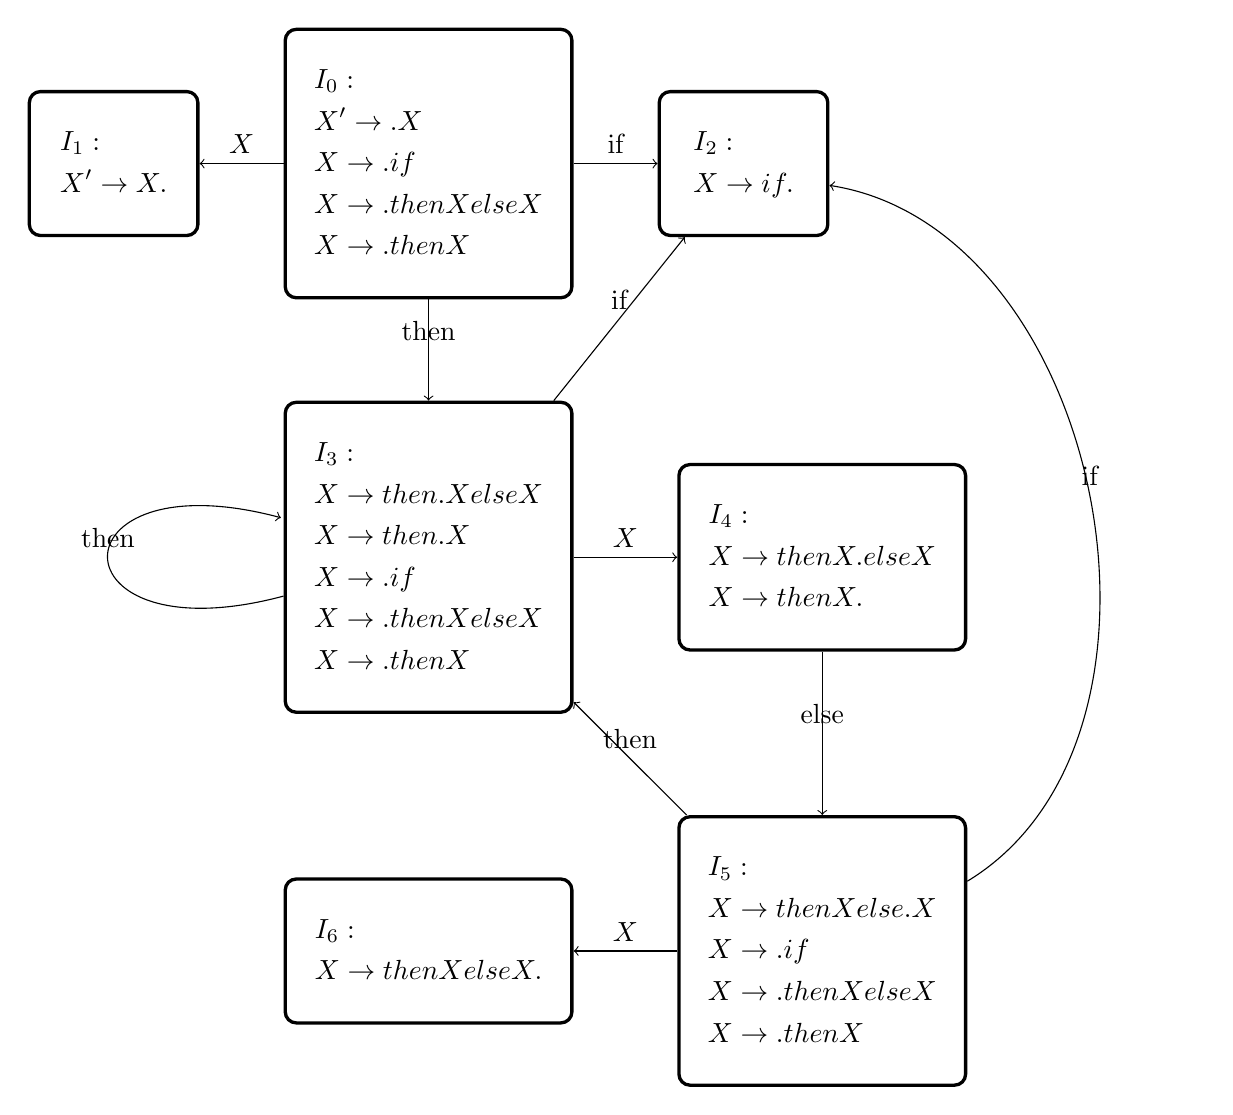
\begin{tikzpicture}
                      \node[state] (I0) {
                        \parbox{3.5cm}{\begin{equation*}\begin{aligned}
                               & I_0:                      \\
                               & X' \rightarrow .X         \\
                               & X \rightarrow .if         \\
                               & X \rightarrow .thenXelseX \\
                               & X \rightarrow .thenX      \\
                            \end{aligned}\end{equation*}}
                      };
                      \node[state, left of=I0, node distance=4cm] (I1){
                        \parbox{2cm}{\begin{equation*}\begin{aligned}
                               & I_1:             \\
                               & X'\rightarrow X. \\
                            \end{aligned}\end{equation*}}
                      };
                      \node[state, right of=I0, node distance=4cm] (I2){
                        \parbox{2cm}{\begin{equation*}\begin{aligned}
                               & I_2:             \\
                               & X\rightarrow if. \\
                            \end{aligned}\end{equation*}}
                      };
                      \node[state, below of=I0, node distance=5cm] (I3){
                        \parbox{3.5cm}{\begin{equation*}\begin{aligned}
                               & I_3:                      \\
                               & X \rightarrow then.XelseX \\
                               & X \rightarrow then.X      \\
                               & X \rightarrow .if         \\
                               & X \rightarrow .thenXelseX \\
                               & X \rightarrow .thenX      \\
                            \end{aligned}\end{equation*}}
                      };
                      \node[state, right of=I3, node distance=5cm] (I4){
                        \parbox{3.5cm}{\begin{equation*}\begin{aligned}
                               & I_4:                      \\
                               & X \rightarrow thenX.elseX \\
                               & X \rightarrow thenX.      \\
                            \end{aligned}\end{equation*}}
                      };
                      \node[state, below of=I4, node distance=5cm] (I5){
                        \parbox{3.5cm}{\begin{equation*}\begin{aligned}
                               & I_5:                      \\
                               & X \rightarrow thenXelse.X \\
                               & X \rightarrow .if         \\
                               & X \rightarrow .thenXelseX \\
                               & X \rightarrow .thenX      \\
                            \end{aligned}\end{equation*}}
                      };
                      \node[state, below of=I3, node distance=5cm] (I6){
                        \parbox{3.5cm}{\begin{equation*}\begin{aligned}
                               & I_6:                      \\
                               & X \rightarrow thenXelseX. \\
                            \end{aligned}\end{equation*}}
                      };
                      \path[->](I0) edge node[above]{$X$}(I1);
                      \path[->](I0) edge node[above]{if}(I2);
                      \path[->](I0) edge node[above]{then} (I3);
                      \path[->](I3) edge node[above]{if} (I2);
                      \path[->](I3) edge[loop left] node[above]{then} (I3);
                      \path[->](I3) edge node[above]{$X$} (I4);
                      \path[->](I4) edge node[above]{else} (I5);
                      \path[->](I5) edge node[above]{$X$} (I6);
                      \path[->](I5) edge[bend right=70] node[above]{if} (I2);
                      \path[->](I5) edge node[above]{then} (I3);
                    \end{tikzpicture}\end{center}
                }
          \item Identify a shift-reduce conflict in this grammar under the
                SLR(1) rules.\\
                \textcolor{blue}{
                  In state 4 ($I_4$), there is a shift-reduce conflict, that when the next input is terminal 'else', it can shift to state 5 ($I_5$), as well as be reduced by $X\rightarrow thenX$.
                }
          \item Assuming that an SLR(1) parser resolves shift-reduce conflicts
                by choosing to shift, show the operation of such a parser on the input
                string \textbf{then then if else then}.\\
                \textcolor{blue}{
                  \begin{tabular}{l r l l}
                    stack                             & input                     & action                      & output            \\
                    \hline
                    0                                 & then then if else then \$ & shift 3                     &                   \\
                    0 then 3                          & then if else then \$      & shift 3                     &                   \\
                    0 then 3 then 3                   & if else then \$           & shift 2                     &                   \\
                    0 then 3 then 3 if 2              & else then \$              & reduce by $X\rightarrow if$ & $X\rightarrow if$ \\
                    0 then 3 then 3 X 4               & else then \$              & shift 5                     &                   \\
                    0 then 3 then 2 X 4 else 5        & then \$                   & shift 3                     &                   \\
                    0 then 3 then 2 X 4 else 5 then 3 & \$                        & error                       &                   \\
                  \end{tabular}
                }
          \item Suppose you can use the \textbf{Bison} type of grammar to specify the priority to reduce the conflict, how
                can you do so? Write the \textbf{Bison} code.\\
                \textcolor{blue}{
                  By adding precendence to token IF and ELSE, respectively correspond to string "if" and "else" in tokenizer. Here's the first part of the parser (.y file).
                }
                \begin{minted}[mathescape, linenos]{c}
/** Your answer here */
%{
#include <stdio.h>
%}
%token IF THEN ELSE
%nonassoc THEN
%nonassoc ELSE
%start X
                \end{minted}

          \item If you can't apply the piority to solve the problem, how can you do it with modified CFG? Write the modified
                CFG.
                \textcolor{blue}{
                  \[\begin{array}{cll}
                      X             & \rightarrow & matchedstmt\ |\ unmatchedstmt                                                          \\
                      matchedstmt   & \rightarrow & \textbf{then}\ matchedstmt\ \textbf{else}\ matchedstmt\ | \textbf{if}                  \\
                      unmatchedstmt & \rightarrow & \textbf{then}\  X\ |\ \textbf{then}\  matchedstatement\  \textbf{else}\  unmatchedstmt
                    \end{array}\]
                }
        \end{enumerate}
\end{enumerate}
\end{document}


